
\documentclass{beamer}
\usecolortheme{dove}
\setbeamertemplate{navigation symbols}{}
\usepackage{amsmath,amssymb,amsfonts,amsthm, multicol, subfigure, color}
\usepackage{bm}
\usepackage{graphicx}
\usepackage{tabularx}
\usepackage{booktabs}
\usepackage{hyperref}
\usepackage{pdfpages}
\usepackage{xcolor}
\definecolor{seagreen}{RGB}{46, 139, 87}
\def\independenT#1#2{\mathrel{\rlap{$#1#2$}\mkern2mu{#1#2}}}
\newcommand\indep{\protect\mathpalette{\protect\independenT}{\perp}}
\def\log{\text{log}}
\newcommand\logit{\text{logit}}
\newcommand\iid{\stackrel{\text{iid}}{\sim}}
\newcommand\E{\text{E}}
\newcommand\V{\text{V}}
\renewcommand\P{\text{P}}
\newcommand{\Cov}{\text{Cov}}
\newcommand{\Cor}{\text{Cor}}
\newcommand\doop{\texttt{do}}
\usepackage{stackrel}
\usepackage{tikz}
\usetikzlibrary{arrows,shapes.arrows,positioning,shapes,patterns,calc}
\newcommand\slideref[1]{\vskip .1cm \tiny \textcolor{gray}{{#1}}}
\newcommand\red[1]{\color{red}#1}
\newcommand\blue[1]{\color{blue}#1}
\newcommand\gray[1]{\color{gray}#1}
\newcommand\seagreen[1]{\color{seagreen}#1}
\newcommand\purple[1]{\color{purple}#1}
\newcommand\orange[1]{\color{orange}#1}
\newcommand\black[1]{\color{black}#1}
\newcommand\white[1]{\color{white}#1}
\newcommand\teal[1]{\color{teal}#1}
\newcommand\magenta[1]{\color{magenta}#1}
\newcommand\Fuchsia[1]{\color{Fuchsia}#1}
\newcommand\BlueGreen[1]{\color{BlueGreen}#1}
\newcommand\bblue[1]{\textcolor{blue}{\textbf{#1}}}
\newcommand\bred[1]{\textcolor{red}{\textbf{#1}}}
\newcommand\bgray[1]{\textcolor{gray}{\textbf{#1}}}
\newcommand\bgreen[1]{\textcolor{seagreen}{\textbf{#1}}}
\newcommand\bref[2]{\href{#1}{\color{blue}{#2}}}
\colorlet{lightgray}{gray!40}
\pgfdeclarelayer{bg}    % declare background layer for tikz
\pgfsetlayers{bg,main} % order layers for tikz
\newcommand\mycite[1]{\begin{scriptsize}\textcolor{darkgray}{(#1)}\end{scriptsize}}
\newcommand{\tcframe}{\frame{
%\small{
\only<1|handout:0>{\tableofcontents}
\only<2|handout:1>{\tableofcontents[currentsubsection]}}
%}
}

\usepackage[round]{natbib}
\bibliographystyle{humannat-mod}
\setbeamertemplate{enumerate items}[default]
\usepackage{mathtools}

\newcommand{\goalsframe}{\begin{frame}{Learning goals for today}
At the end of class, you will be able to:
\begin{enumerate}
\item Reason about the sequential ignorability assumption
\item Apply inverse probability weighting to treatments over time
\end{enumerate} \vskip .2in
\end{frame}}

\title{16. Treatments in many time periods.\\What to do.}
\author{Ian Lundberg\\Cornell Info 6751: Causal Inference in Observational Settings\\Fall 2022}
\date{18 Oct 2022}

\begin{document}

\maketitle

\goalsframe

\begin{frame}[t]{Identification: The adjustment set}
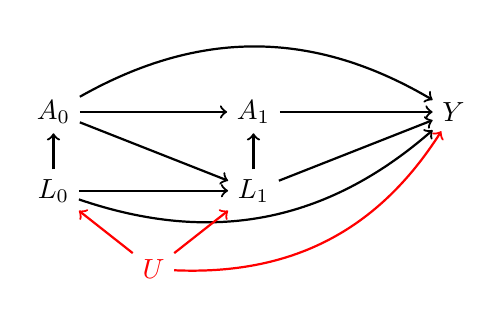
\begin{tikzpicture}[x = 1in]
\node (y) at (2,0) {$Y$};
\node[red] (u) at (.5,-2) {$U$};
\node (l0) at (0,-1) {$L_0$};
\node (a0) at (0,0) {$A_0$};
\node (l1) at (1,-1) {$L_1$};
\draw[->, thick] (l0) -- (a0);
\draw[->, thick] (l0) to[bend right] (y);
\draw[->, thick] (a0) to[bend left] (y);
\node (a1) at (1,0) {$A_1$};
\draw[->, thick] (a0) -- (a1);
\draw[->, thick] (l0) -- (l1);
\draw[->, thick] (a0) -- (l1);
\draw[->, thick] (l1) -- (a1);
\draw[->, thick] (l1) -- (y);
\draw[->, thick] (a1) -- (y);
\draw[->, thick, red] (u) -- (l0);
\draw[->, thick, red] (u) -- (l1);
\draw[->, thick, red] (u) to[bend right] (y);
\end{tikzpicture} \vskip .2in
A joint adjustment set for $\bar{A}$ is doomed \pause
\begin{itemize}
\item What happens if you adjust for $L_1$? \pause
\begin{itemize}
\item You block a causal path: $A_0\rightarrow \boxed{L_1}\rightarrow Y$
\item You open a backdoor path: $A_0 \rightarrow \boxed{L_1}\leftarrow U\rightarrow Y$
\end{itemize} \pause
\item What happens if you don't adjust for $L_1$? \pause
\begin{itemize}
\item A backdoor path remains: $A_1 \leftarrow L_1\rightarrow Y$
\end{itemize} 
\end{itemize} \pause
To proceed, we need a different adjustment set in each time period
\end{frame}

\begin{frame}{Notation}

\begin{itemize}
\item $\bar{A}_k = (A_0,A_1,\dots,A_k)$ \hfill treatments up to time $k$
\item $\bar{L}_k = (L_0,L_1,\dots,L_k)$ \hfill confounders up to time $k$
\item $g()$ \hfill treatment strategy
\item $Y^g$ \hfill potential outcome under that strategy
\end{itemize}

\end{frame}

\begin{frame}[t]{Identification: Sequential ignorability}
\onslide<2-6>{
\begin{center}
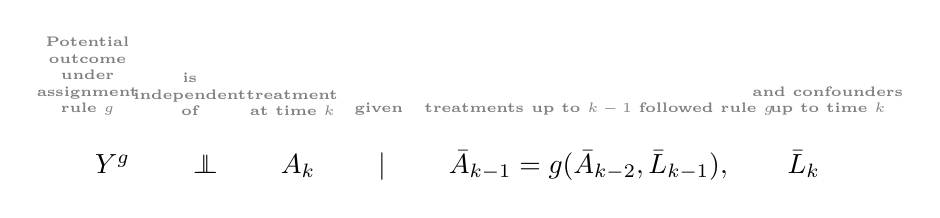
\begin{tikzpicture}[y = .2in]
\node at (0,0) {$Y^g \qquad \indep \qquad A_k\qquad \mid \qquad \bar{A}_{k-1} = g(\bar{A}_{k-2}, \bar{L}_{k-1}), \qquad \bar{L}_k$};
\node[anchor = south, font = {\tiny\bf}, gray, align = center] at (-4.7,1) {Potential\\outcome\\under\\assignment\\rule $g$};
\node[anchor = south, font = {\tiny\bf}, gray, align = center] at (-3.4,1) {is\\independent\\of};
\node[anchor = south, font = {\tiny\bf}, gray, align = center] at (-2.1,1) {treatment\\at time $k$};
\node[anchor = south, font = {\tiny\bf}, gray, align = center] at (-1,1) {given};
\node[anchor = south, font = {\tiny\bf}, gray, align = center] at (1.8,1) {treatments up to $k-1$ followed rule $g$};
\node[anchor = south, font = {\tiny\bf}, gray, align = center] at (4.7,1) {and confounders\\up to time $k$};
\end{tikzpicture}
\end{center}
for all assignment rules $g$ and time periods $k = 1,\dots,K$
\begin{center}
\onslide<3-6>{
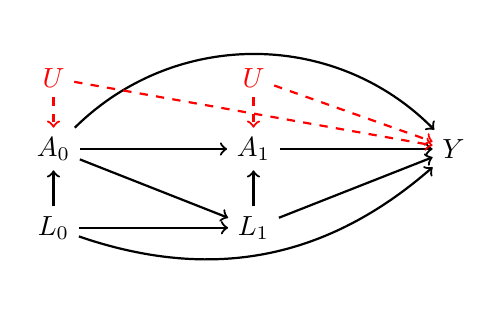
\begin{tikzpicture}[x = 1in]
\node (y) at (2,0) {$Y$};
\node (l0) at (0,-1) {$L_0$};
\node (a0) at (0,0) {$A_0$};
\node (l1) at (1,-1) {$L_1$};
\draw[->, thick] (l0) -- (a0);
\draw[->, thick] (l0) to[bend right] (y);
\draw[->, thick] (a0) to[bend left = 45] (y);
\node (a1) at (1,0) {$A_1$};
\draw[->, thick] (a0) -- (a1);
\draw[->, thick] (l0) -- (l1);
\draw[->, thick] (a0) -- (l1);
\draw[->, thick] (l1) -- (a1);
\draw[->, thick] (l1) -- (y);
\draw[->, thick] (a1) -- (y);
\onslide<4>{
\node[red] (u) at (0,.9) {$U$};
\draw[->, thick, red, dashed] (u) -- (a0);
\draw[->, thick, red, dashed] (u) -- (y);
}
\onslide<5>{
\node[red] (u) at (1,.9) {$U$};
\draw[->, thick, red, dashed] (u) -- (a1);
\draw[->, thick, red, dashed] (u) -- (y);
}
\end{tikzpicture}
}
\end{center}
}

\end{frame}

\begin{frame}{Estimation: Two strategies}

\begin{enumerate}
\item Inverse probability weighting (+ marginal structural models)
\item Structural nested mean models (coming next class)
\end{enumerate}

\end{frame}

\begin{frame}{Inverse probability weighting: DAG motivation} \pause

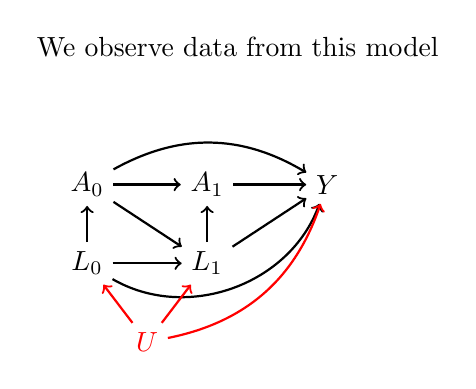
\begin{tikzpicture}[x = .6in]
\node[anchor = north west] at (-.5,2) {We observe data from this model};
\node (y) at (2,0) {$Y$};
\node[red] (u) at (.5,-2) {$U$};
\node (l0) at (0,-1) {$L_0$};
\node (a0) at (0,0) {$A_0$};
\node (l1) at (1,-1) {$L_1$};
\draw[->, thick] (l0) -- (a0);
\draw[->, thick] (l0) to[bend right = 50] (y);
\draw[->, thick] (a0) to[bend left] (y);
\node (a1) at (1,0) {$A_1$};
\draw[->, thick] (a0) -- (a1);
\draw[->, thick] (l0) -- (l1);
\draw[->, thick] (a0) -- (l1);
\draw[->, thick] (l1) -- (a1);
\draw[->, thick] (l1) -- (y);
\draw[->, thick] (a1) -- (y);
\draw[->, thick, red] (u) -- (l0);
\draw[->, thick, red] (u) -- (l1);
\draw[->, thick, red] (u) to[bend right] (y);
\end{tikzpicture} \pause \qquad 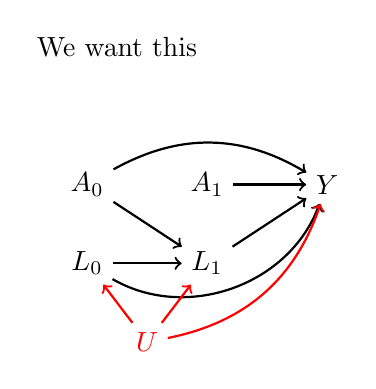
\begin{tikzpicture}[x = .6in]
\node[anchor = north west, align = left] at (-.5,2) {We want this};
\node (y) at (2,0) {$Y$};
\node[red] (u) at (.5,-2) {$U$};
\node (l0) at (0,-1) {$L_0$};
\node (a0) at (0,0) {$A_0$};
\node (l1) at (1,-1) {$L_1$};
%\draw[->, thick, dashed] (l0) -- (a0);
\draw[->, thick] (l0) to[bend right = 50] (y);
\draw[->, thick] (a0) to[bend left] (y);
\node (a1) at (1,0) {$A_1$};
%\draw[->, thick, dashed] (a0) -- (a1);
\draw[->, thick] (l0) -- (l1);
\draw[->, thick] (a0) -- (l1);
%\draw[->, thick, dashed] (l1) -- (a1);
\draw[->, thick] (l1) -- (y);
\draw[->, thick] (a1) -- (y);
\draw[->, thick, red] (u) -- (l0);
\draw[->, thick, red] (u) -- (l1);
\draw[->, thick, red] (u) to[bend right] (y);
\end{tikzpicture} \pause \vskip .1in
\begin{enumerate}
\item How would you weight to estimate the effect of $A_0$?
\item How would you weight to estimate the effect of $A_1$?
\end{enumerate} \vskip .1in
We will combine these

\end{frame}

\begin{frame}{Inverse probability weighting}

In time 0, define an inverse probability of treatment weight
$$W^{A_0} = \frac{1}{\P(A_0\mid L_0)}$$
such that $A_0$ does not depend on $L_0$ after weighting \vskip .1in \pause
In time 1, do it again
$$W^{A_1} = \frac{1}{\P(A_0\mid \bar{A}_{k-1}, \bar{L}_1)}$$ \vskip .1in \pause
Continue through all time periods. \vskip .3in \pause
Define the overall weight as the product
$$W^{\bar{A}} = \prod_{k=0}^K \frac{1}{\P(A_k\mid \bar{A}_{k-1},\bar{L}_k)}$$

\end{frame}

\begin{frame}{Inverse probability weighting}
$$W^{\bar{A}} = \prod_{k=0}^K \frac{1}{\P(A_k\mid \bar{A}_{k-1},\bar{L}_k)}$$
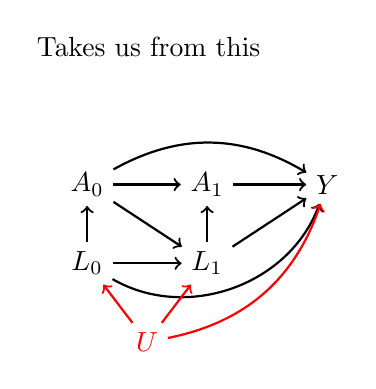
\begin{tikzpicture}[x = .6in]
\node[anchor = north west] at (-.5,2) {Takes us from this};
\node (y) at (2,0) {$Y$};
\node[red] (u) at (.5,-2) {$U$};
\node (l0) at (0,-1) {$L_0$};
\node (a0) at (0,0) {$A_0$};
\node (l1) at (1,-1) {$L_1$};
\draw[->, thick] (l0) -- (a0);
\draw[->, thick] (l0) to[bend right = 50] (y);
\draw[->, thick] (a0) to[bend left] (y);
\node (a1) at (1,0) {$A_1$};
\draw[->, thick] (a0) -- (a1);
\draw[->, thick] (l0) -- (l1);
\draw[->, thick] (a0) -- (l1);
\draw[->, thick] (l1) -- (a1);
\draw[->, thick] (l1) -- (y);
\draw[->, thick] (a1) -- (y);
\draw[->, thick, red] (u) -- (l0);
\draw[->, thick, red] (u) -- (l1);
\draw[->, thick, red] (u) to[bend right] (y);
\end{tikzpicture} 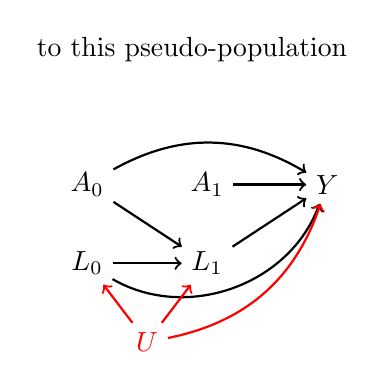
\begin{tikzpicture}[x = .6in]
\node[anchor = north west, align = left] at (-.5,2) {to this pseudo-population};
\node (y) at (2,0) {$Y$};
\node[red] (u) at (.5,-2) {$U$};
\node (l0) at (0,-1) {$L_0$};
\node (a0) at (0,0) {$A_0$};
\node (l1) at (1,-1) {$L_1$}; 
%\draw[->, thick, dashed] (l0) -- (a0);
\draw[->, thick] (l0) to[bend right = 50] (y);
\draw[->, thick] (a0) to[bend left] (y);
\node (a1) at (1,0) {$A_1$};
%\draw[->, thick, dashed] (a0) -- (a1);
\draw[->, thick] (l0) -- (l1);
\draw[->, thick] (a0) -- (l1);
%\draw[->, thick, dashed] (l1) -- (a1);
\draw[->, thick] (l1) -- (y);
\draw[->, thick] (a1) -- (y);
\draw[->, thick, red] (u) -- (l0);
\draw[->, thick, red] (u) -- (l1);
\draw[->, thick, red] (u) to[bend right] (y);
\end{tikzpicture}
\end{frame}

\begin{frame}{Inverse probability weighting with marginal structural models}

Finally, we can put a model on top of the weighting.

$$\E(Y^{\bar{a}}) = \E(Y\mid \bar{A} = \bar{a}) = h(\bar{a})$$
for some function $h()$ that pools information. \vskip .2in
\bgray{Example:} Outcomes depend on the proportion of periods treated
$$h(\bar{a}) = \frac{1}{K + 1}\sum_{k=0}^K a_k$$

\end{frame}

\goalsframe

\begin{frame}{Real example: Neighborhood disadvantage}

Wodtke, G. T., Harding, D. J., \& Elwert, F. (2011). \bref{https://doi.org/10.1177/0003122411420816}{Neighborhood effects in temporal perspective: The impact of long-term exposure to concentrated disadvantage on high school graduation.} American Sociological Review, 76(5), 713-736.

\end{frame}

\begin{frame}{Real example: Neighborhood disadvantage}{Wodtke et al. 2011}

How does the neighborhood in which a child lives affect that child's probability of high school completion? \pause

\begin{itemize}
\item Define a neighborhood as a Census tract \pause
\item Score that neighborhood along several dimensions
\begin{itemize}
\item poverty
\item unemployment
\item welfare receipt
\item female-headed households
\item education
\item occupational structure
\end{itemize} \pause
\item Scale by the first principle component \pause
\item Categorize in 5 quintiles \pause
\end{itemize}
This 5-value treatment is ``neighborhood disadvantage''

\end{frame}

\begin{frame}{Real example: Neighborhood disadvantage}{Wodtke et al. 2011}

Neighborhoods are experienced over time:
$$\bar{a}$$
is a trajectory of neighborhood disadvantage over ages $2,3,\dots,17$ \vskip .2in
The authors study the effect of neighborhood disadvantage, \\
\begin{center}
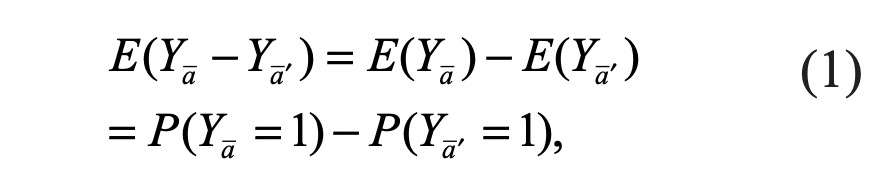
\includegraphics[width = .5\textwidth]{figures/whe_eq1}
\end{center}
Example:\\
$\bar{a}$ is residence in the most advantaged neighborhood each year\\and\\$\bar{a'}$ is residence in the most disadvantaged neighborhood each year
\end{frame}

\begin{frame}{Real example: Neighborhood disadvantage}{Wodtke et al. 2011}

Problem: Neighborhoods $A_1$ shape family characteristics $L_2$, which confound where people live in the future $A_2$ \vskip .1in

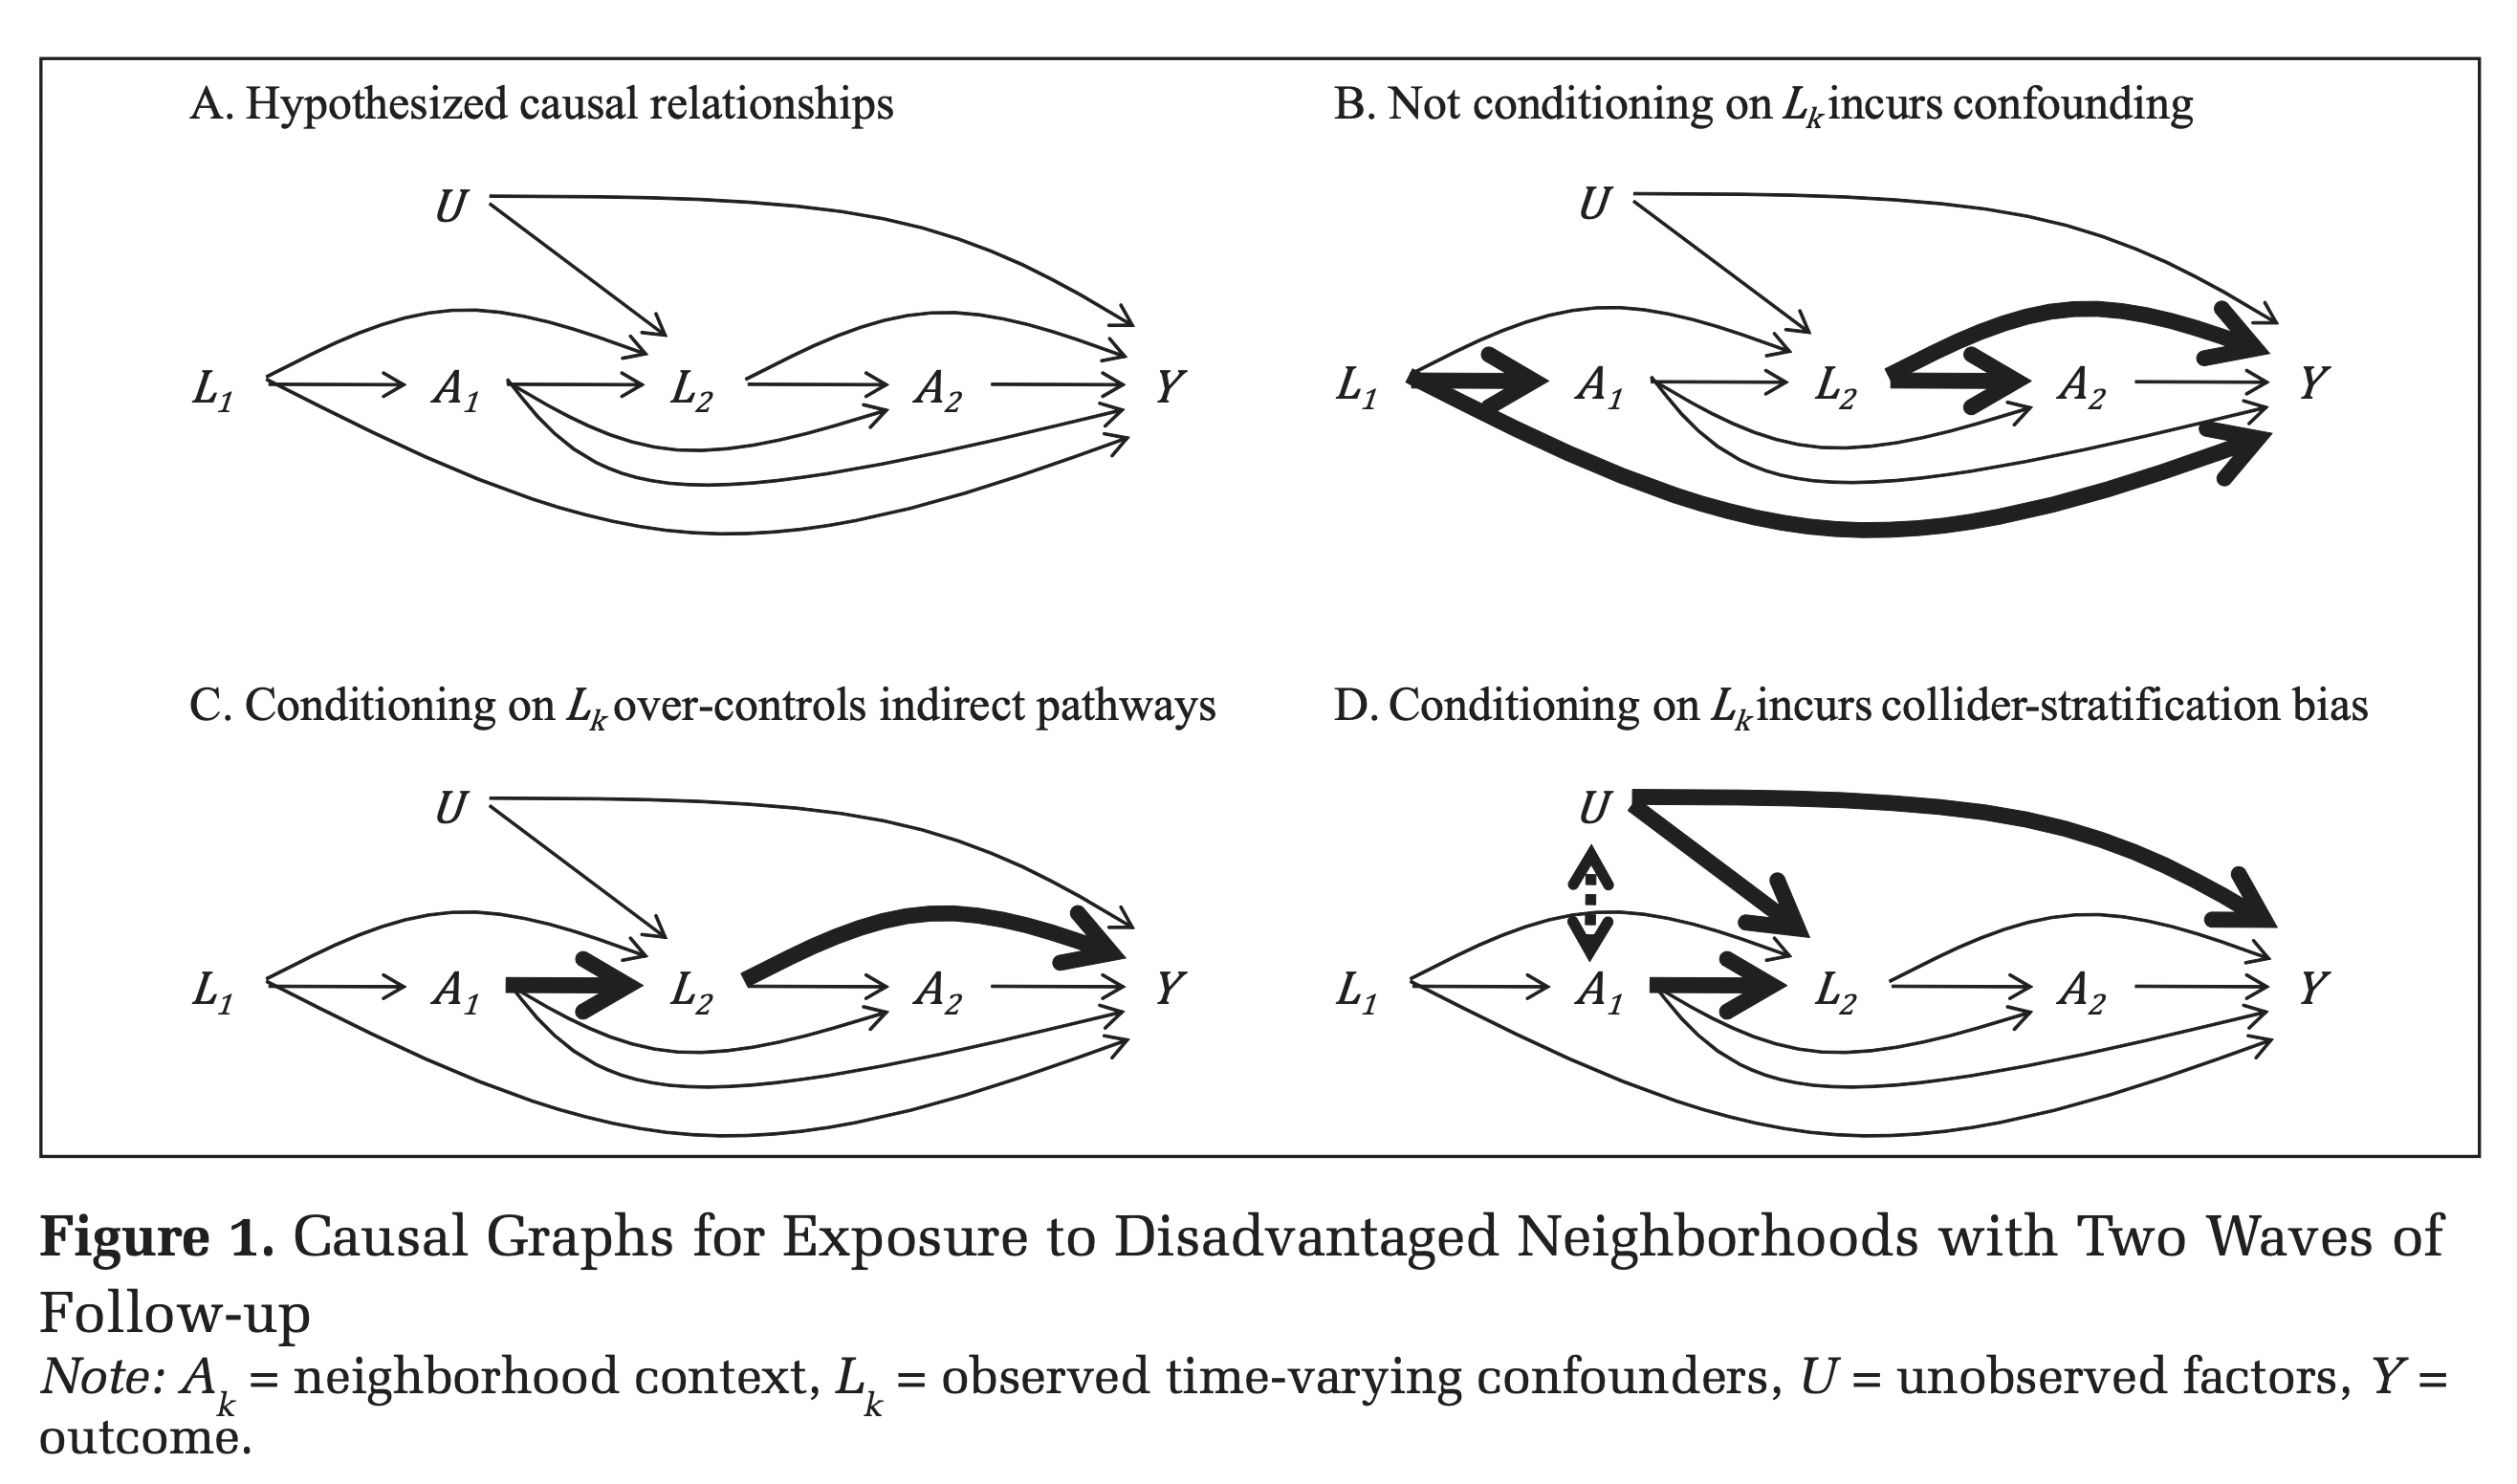
\includegraphics[width = \textwidth]{figures/whe_fig1}

\end{frame}

\begin{frame}%{Real example: Neighborhood disadvantage}{Wodtke et al. 2011}
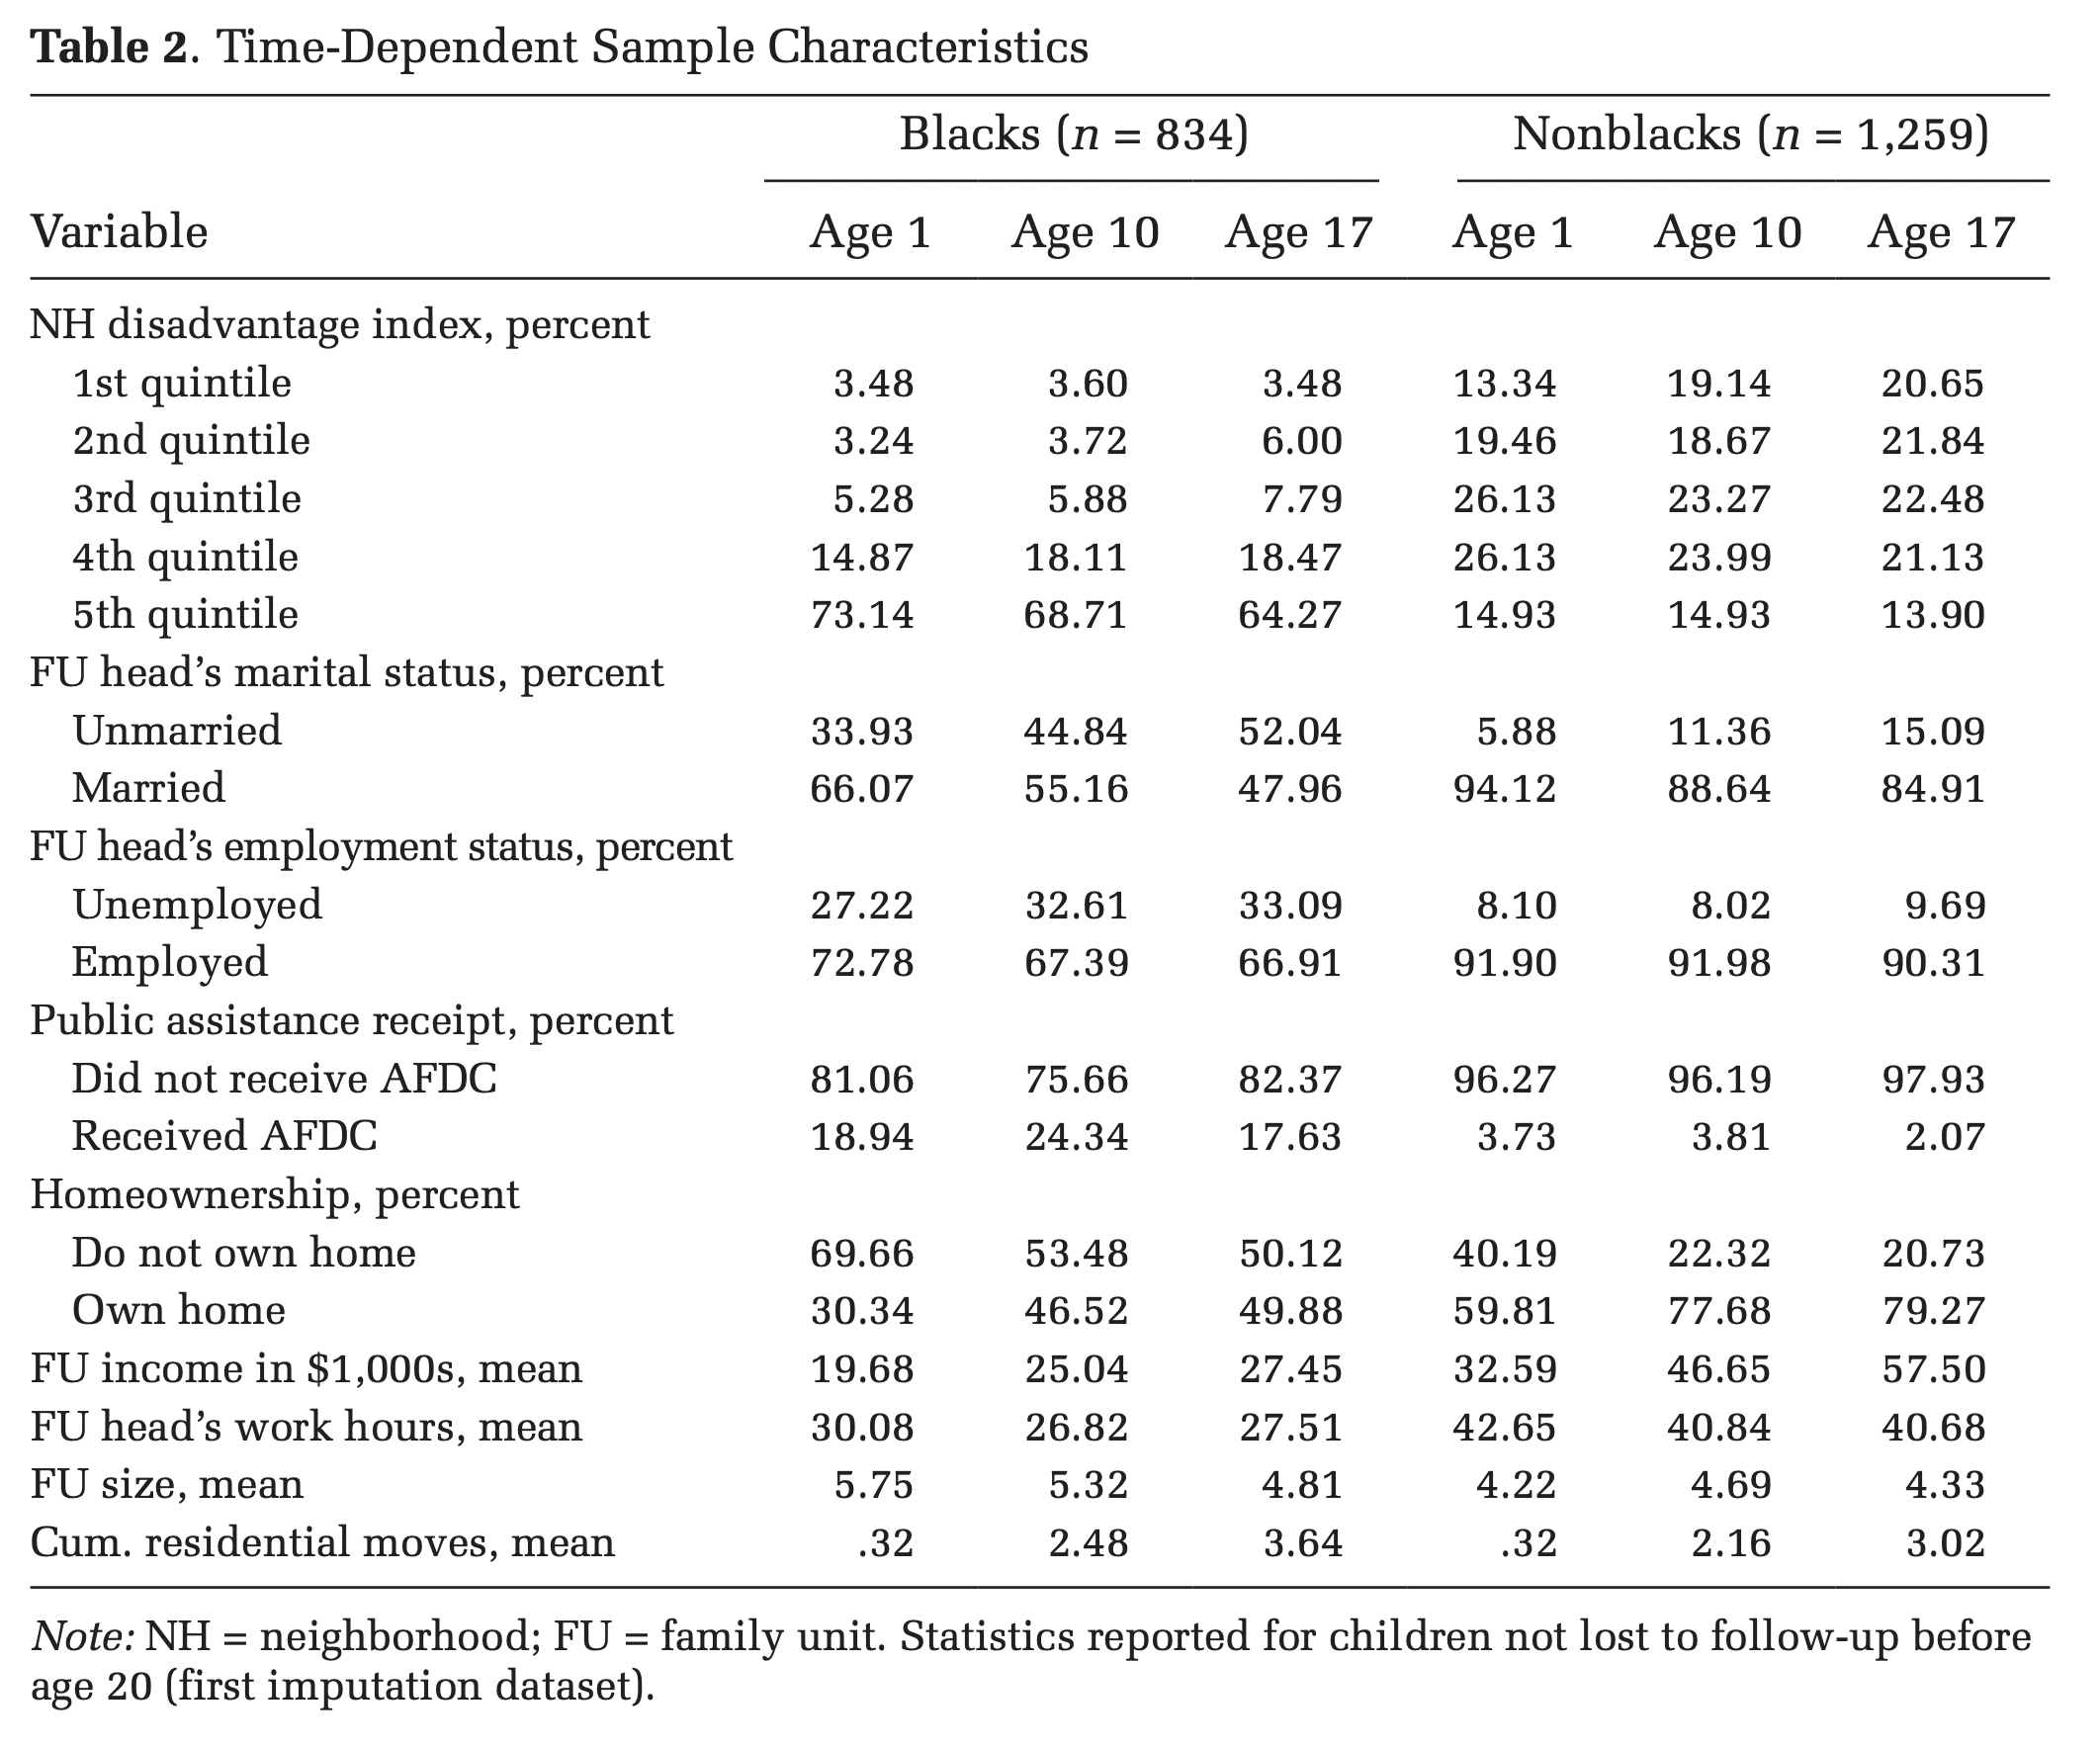
\includegraphics[width = \textwidth]{figures/whe_table3}
\end{frame}

\begin{frame}{Real example: Neighborhood disadvantage}{Wodtke et al. 2011}

Problem: Neighborhoods $A_1$ shape family characteristics $L_2$, which confound where people live in the future $A_2$ \vskip .1in

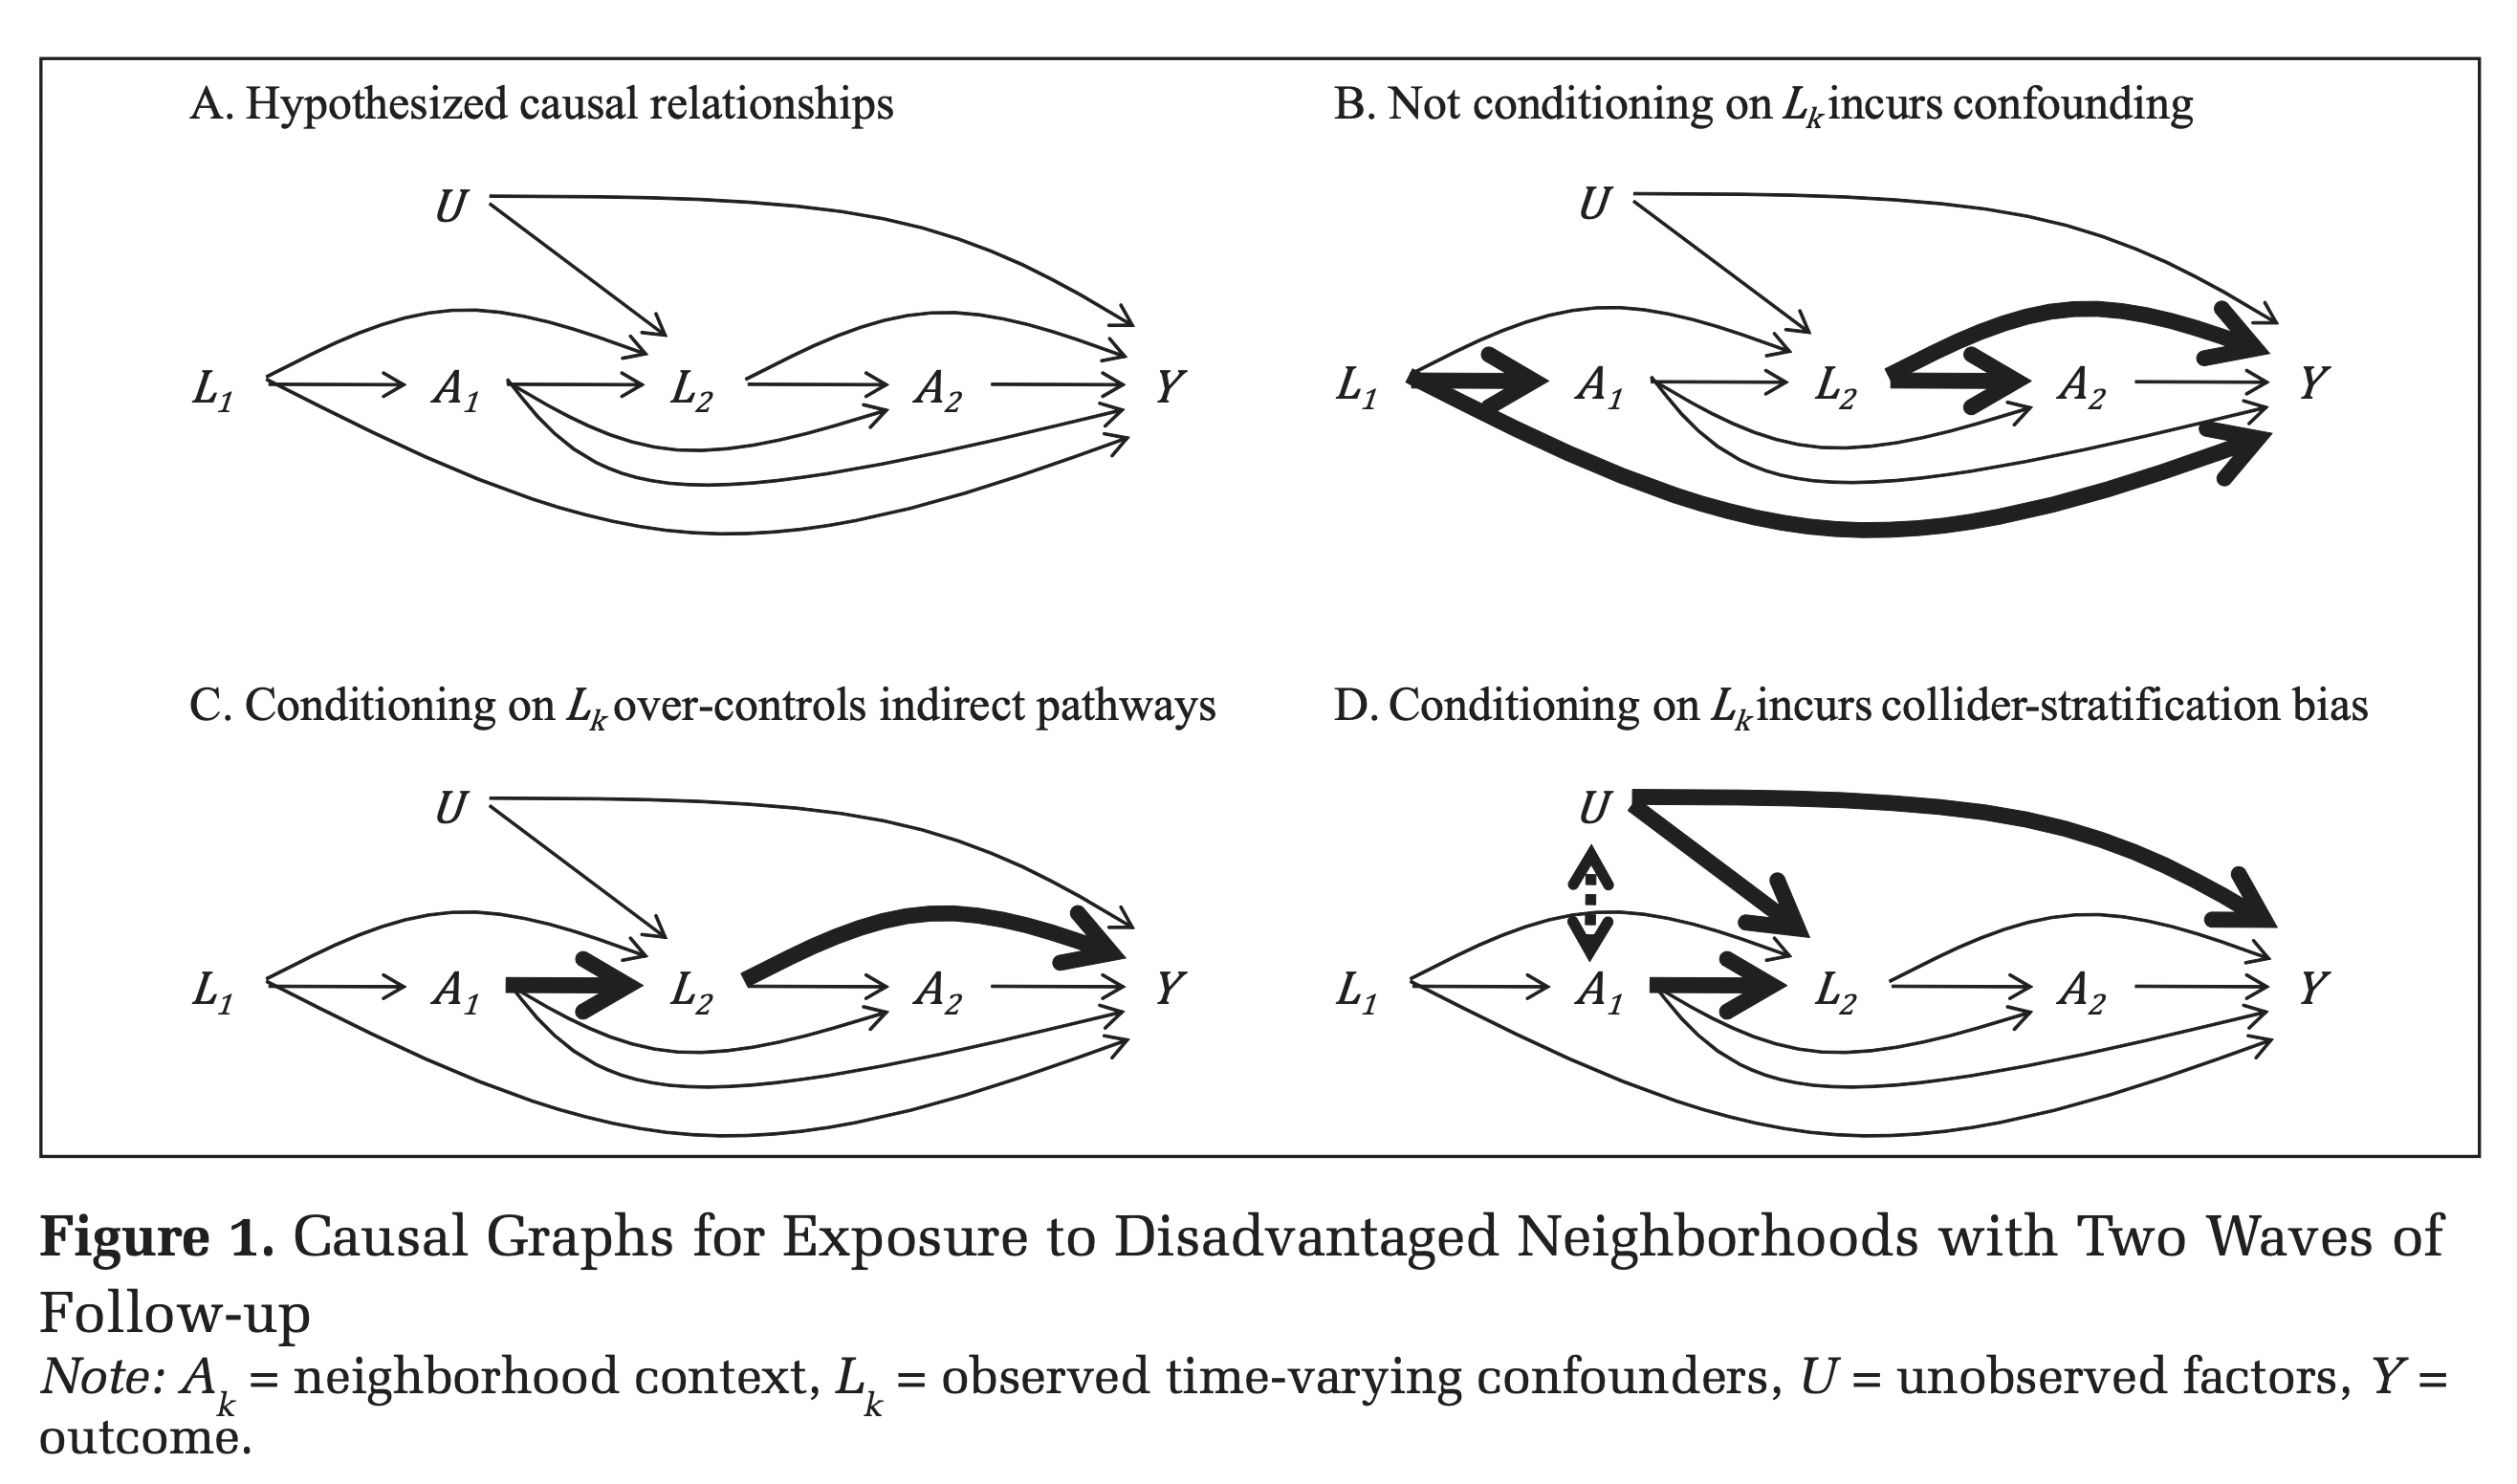
\includegraphics[width = \textwidth]{figures/whe_fig1}

\end{frame}

\begin{frame}{Real example: Neighborhood disadvantage}{Wodtke et al. 2011}

Solution: MSM-IPW \vskip .1in

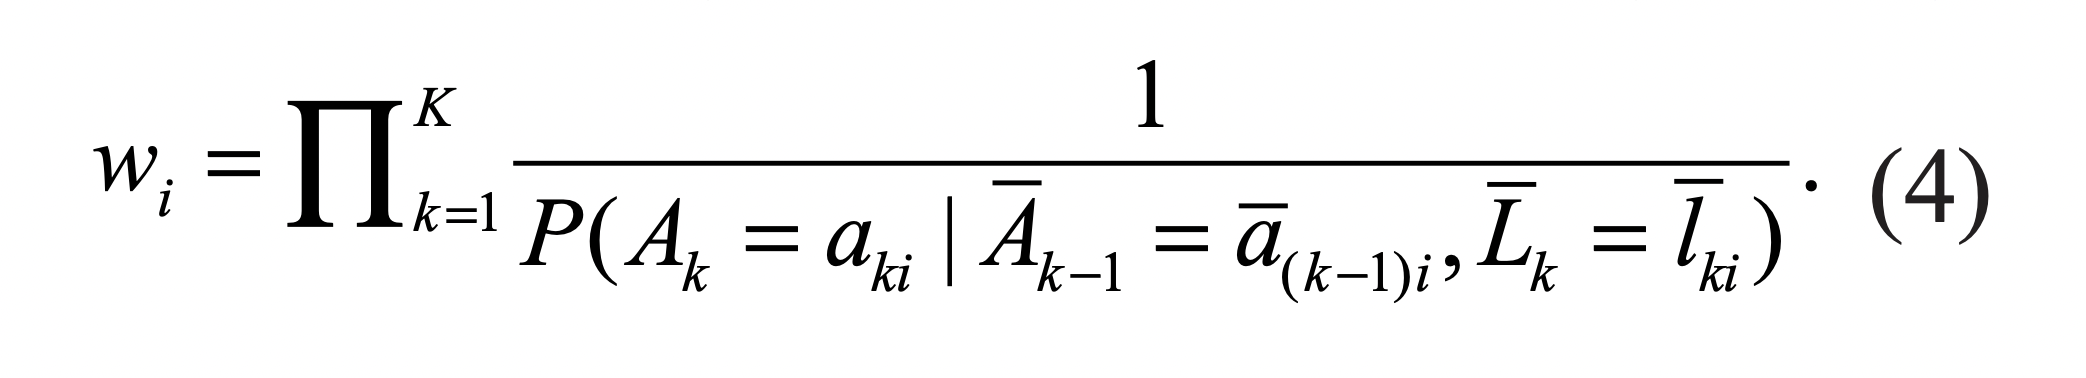
\includegraphics[width = \textwidth]{figures/whe_eq4} \vskip .2in

Also with stabilized weights \vskip .1in

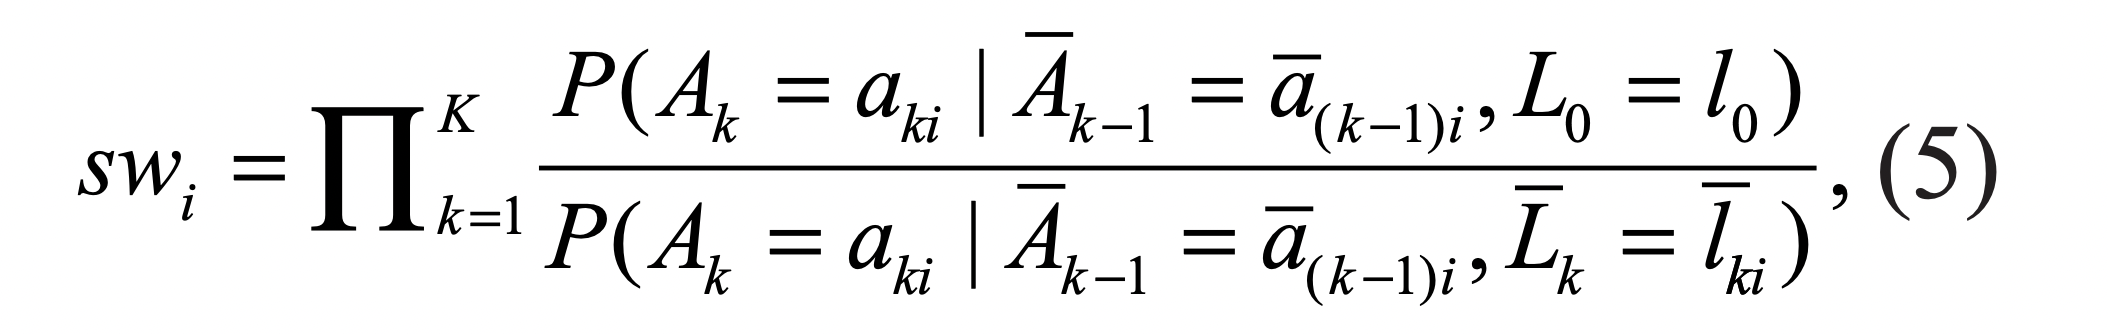
\includegraphics[width = \textwidth]{figures/whe_eq5}

\end{frame}

\begin{frame}{Real example: Neighborhood disadvantage}{Wodtke et al. 2011}
Marginal structural model: Logit
\begin{itemize}
\item 5-category treatment entered numerically
\item Baseline covariates included due to stabilized weights
\item Weights adjust for time-varying confounding
\end{itemize}
\end{frame}

\begin{frame}{Real example: Neighborhood disadvantage}{Wodtke et al. 2011}

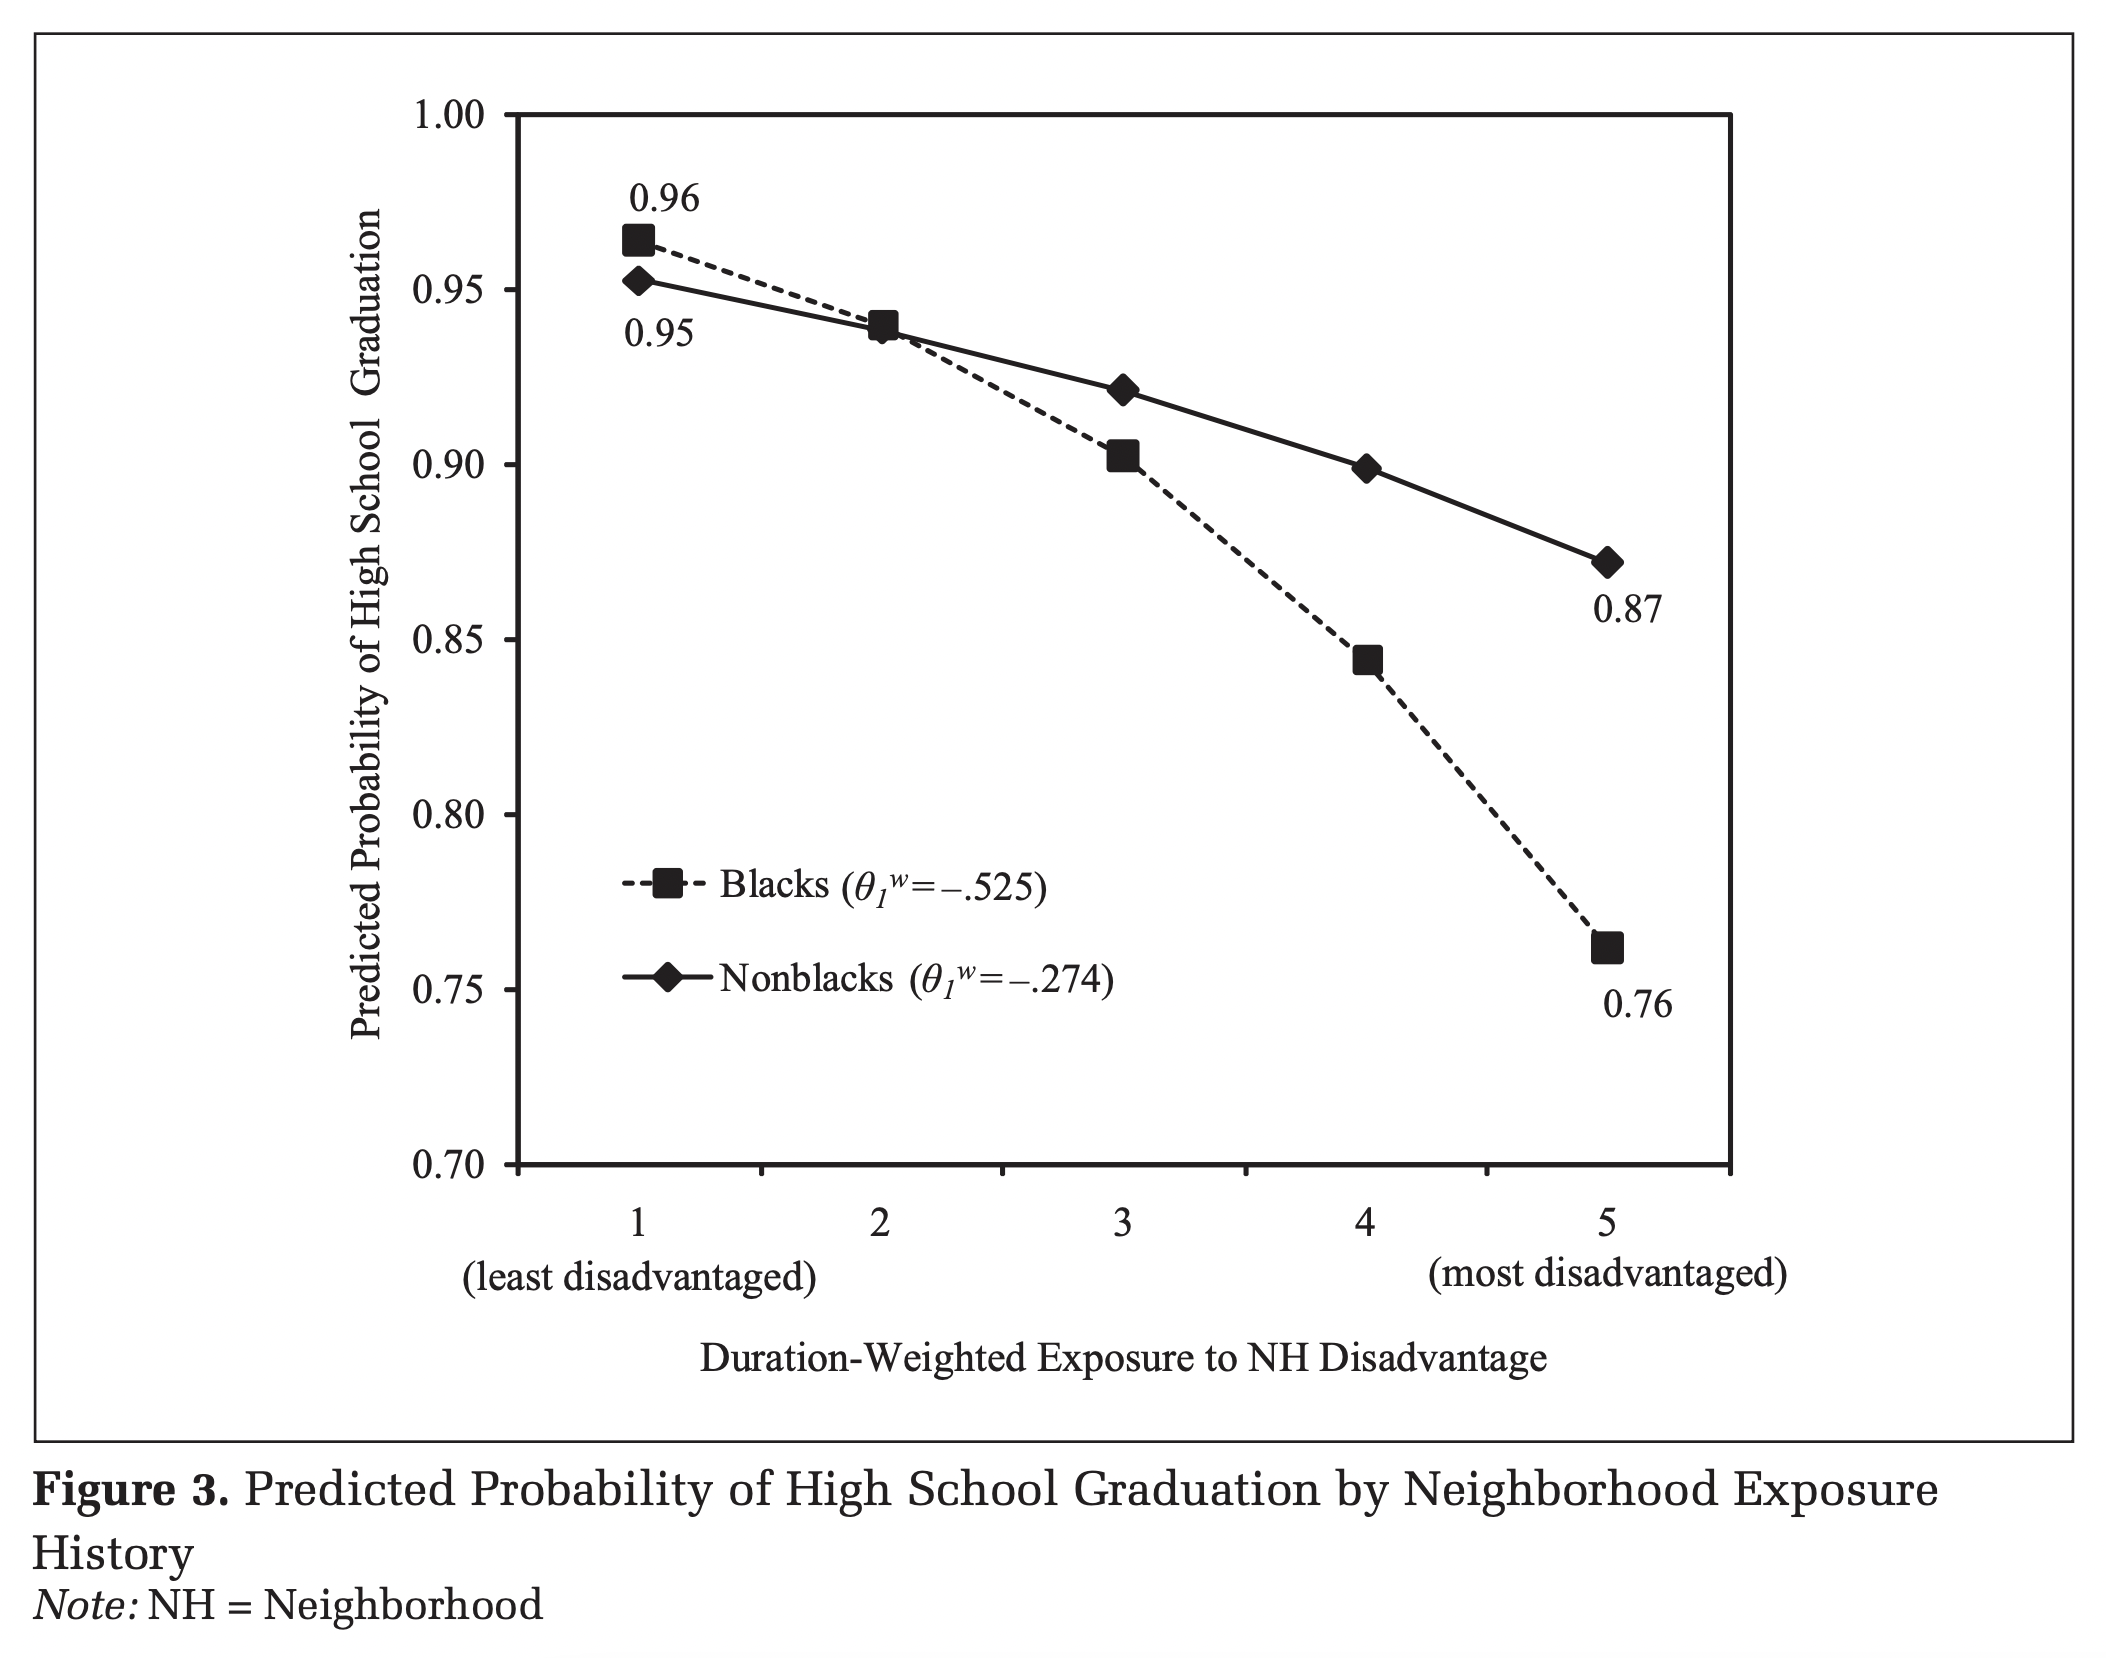
\includegraphics[width = .9\textwidth]{figures/whe_fig3}

\end{frame}

\goalsframe

\begin{frame}{Let me know what you are thinking}

\begin{huge} \bref{https://tinyurl.com/CausalQuestions}{tinyurl.com/CausalQuestions} \end{huge}
\vskip .7in

Office hours TTh 11am-12pm and at \bref{https://calendly.com/ianlundberg/office-hours}{calendly.com/ianlundberg/office-hours}\\Come say hi!

\end{frame}

\end{document}